\documentclass[autodetect-engine, dvipdfmx-if-dvi, ja=standard]{bxjsarticle}

\usepackage{setspace}        % 行間設定に必要
\usepackage{titlesec}        % titleformatの設定に必要
\usepackage{multicol}        % 2段組みにする
\usepackage{type1cm}         % fontsizeのエラー回避
\usepackage{graphicx}        % 図を表示するのに必要
\usepackage{color}           % jpgなどを表示するのに必要
\usepackage{here}            % 図の配置位置を強制する
\usepackage{amsmath,amssymb} % 数学記号を出すのに必要

% 余白の設定
\setlength{\textheight}{\paperheight}   % 紙面縦幅を本文領域にする(BOTTOM=-TOP)
\setlength{\topmargin}{-15.4truemm}     % 上の余白を10mm(=1inch-15.4mm)に
\addtolength{\topmargin}{-\headheight}  %
\addtolength{\topmargin}{-\headsep}     % ヘッダの分だけ本文領域を移動させる
\addtolength{\textheight}{-20truemm}    % 下の余白も10mm
\setlength{\textwidth}{\paperwidth}     % 紙面横幅を本文領域にする(RIGHT=-LEFT)
\setlength{\oddsidemargin}{-5.4truemm}  % 奇数ページの左の余白を20mm(=1inch-5.4mm)に
\setlength{\evensidemargin}{-5.4truemm} % 偶数数ページの左の余白を20mm(=1inch-5.4mm)に
\addtolength{\textwidth}{-40truemm}     % 右の余白も20mm

% sectionのマージンを調整
\makeatletter
  \renewcommand{\section}{%
    \@startsection{section}{1}{\z@}%
    {0.1\Cvs}{0.1\Cvs}%
    {\normalfont\large\headfont\raggedright}}
\makeatother

% その他設定
\parindent = 0pt  % 行頭の字下げをしない
\setstretch{1.0}  % 行間は1文字分
\pagestyle{empty} % ページ番号を消す
\titleformat*{\section}{\fontsize{11.041pt}{16.562pt}\selectfont \bf}

\begin{document}
\begin{center}
    \fontsize{14.053pt}{21.079pt}\selectfont
    {\bf MATLAB/SimulinkによるRADAR計測システムの開発}\\

    \fontsize{11.041pt}{16.562pt}\selectfont
    佐藤\ 凌雅\ (秋田研究室)
\end{center}


\begin{multicols}{2}
\fontsize{10.539pt}{15.809pt}\selectfont

\section{緒言}
 自動車の走行時に生じる上下方向の振動を抑制する装置としてアクティブサスペンションが開発され,市販車に装備されるまでにその技術は進歩している.しかし,その多くはストロークセンサや加速度センサーがバネ下の動きを検知してから作動するもので,車両が段差に侵入した際の最初の衝撃を完全に吸収できない.そこで,車載センサを用いて路面の状態を測定し,車体に衝撃が加わるタイミングでサスペンションを調整することにより,既存のアクティブサスペンション技術では吸収しきれない最初の衝撃を軽減できると考える.\\
 本研究では,このアクティブサスペンションの動作判定の前段として,路面の段差検知システムの実現を目的とする.提案するシステムはRADARを用いて路面を常に監視し,車両前方の段差の有無を検出する.また,システム構築にはMATLAB/Simulinkを用いたモデルベース開発を採用し,ソフトウェア設計の効率向上を図った.

\section{本論}
 本研究では路面の状態を計測するRADARとしてAcconeer社製のXC112/XR112評価キットを使用した.この評価キットを分解組立型電気自動車PIUSの前方に取り付け,本校敷地内を走行しデータを取得した.センサからの距離別の電波の反射強度が得られる.反射強度のピークの位置が物体,すなわち,路面までの距離となる.RADARから得られるデータの例を図\ref{fig:abst_demo}に示す.この例では,0.205mの位置に反射強度のピークが存在するため,地面との距離は0.205mであると推測できる.
\begin{figure}[H]
  \centering
  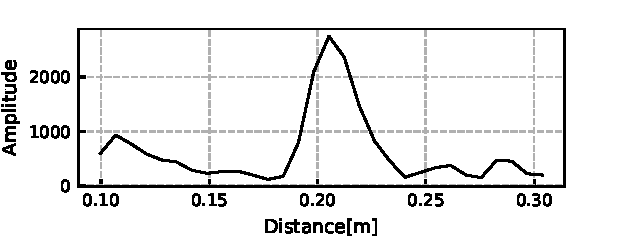
\includegraphics[width=8cm]{../thesis/fig/abst_demo.pdf}
  \caption{RADARから得られるデータの例}
  \label{fig:abst_demo}
\end{figure}

 このRADARのデータから路面の段差の有無を検出するためにMATLAB/Simulink上で図\ref{fig:system_block}のような信号処理アルゴリズムを構築した.\\
 まず,RADARの測定データをMATLABから配列形式で読み込む(1.).電波は自由空間で距離の2乗に比例して減衰するため,それを補償する(2.).その後,ピークが現れてるデータのインデックスを選択し(3.),インデックス番号を実際の距離の単位に変換する(4.).得られた路面までの距離を微分し(5.),微分値が閾値を超えた場合は段差の検知とみなす(6.).
\begin{figure}[H]
  \centering
  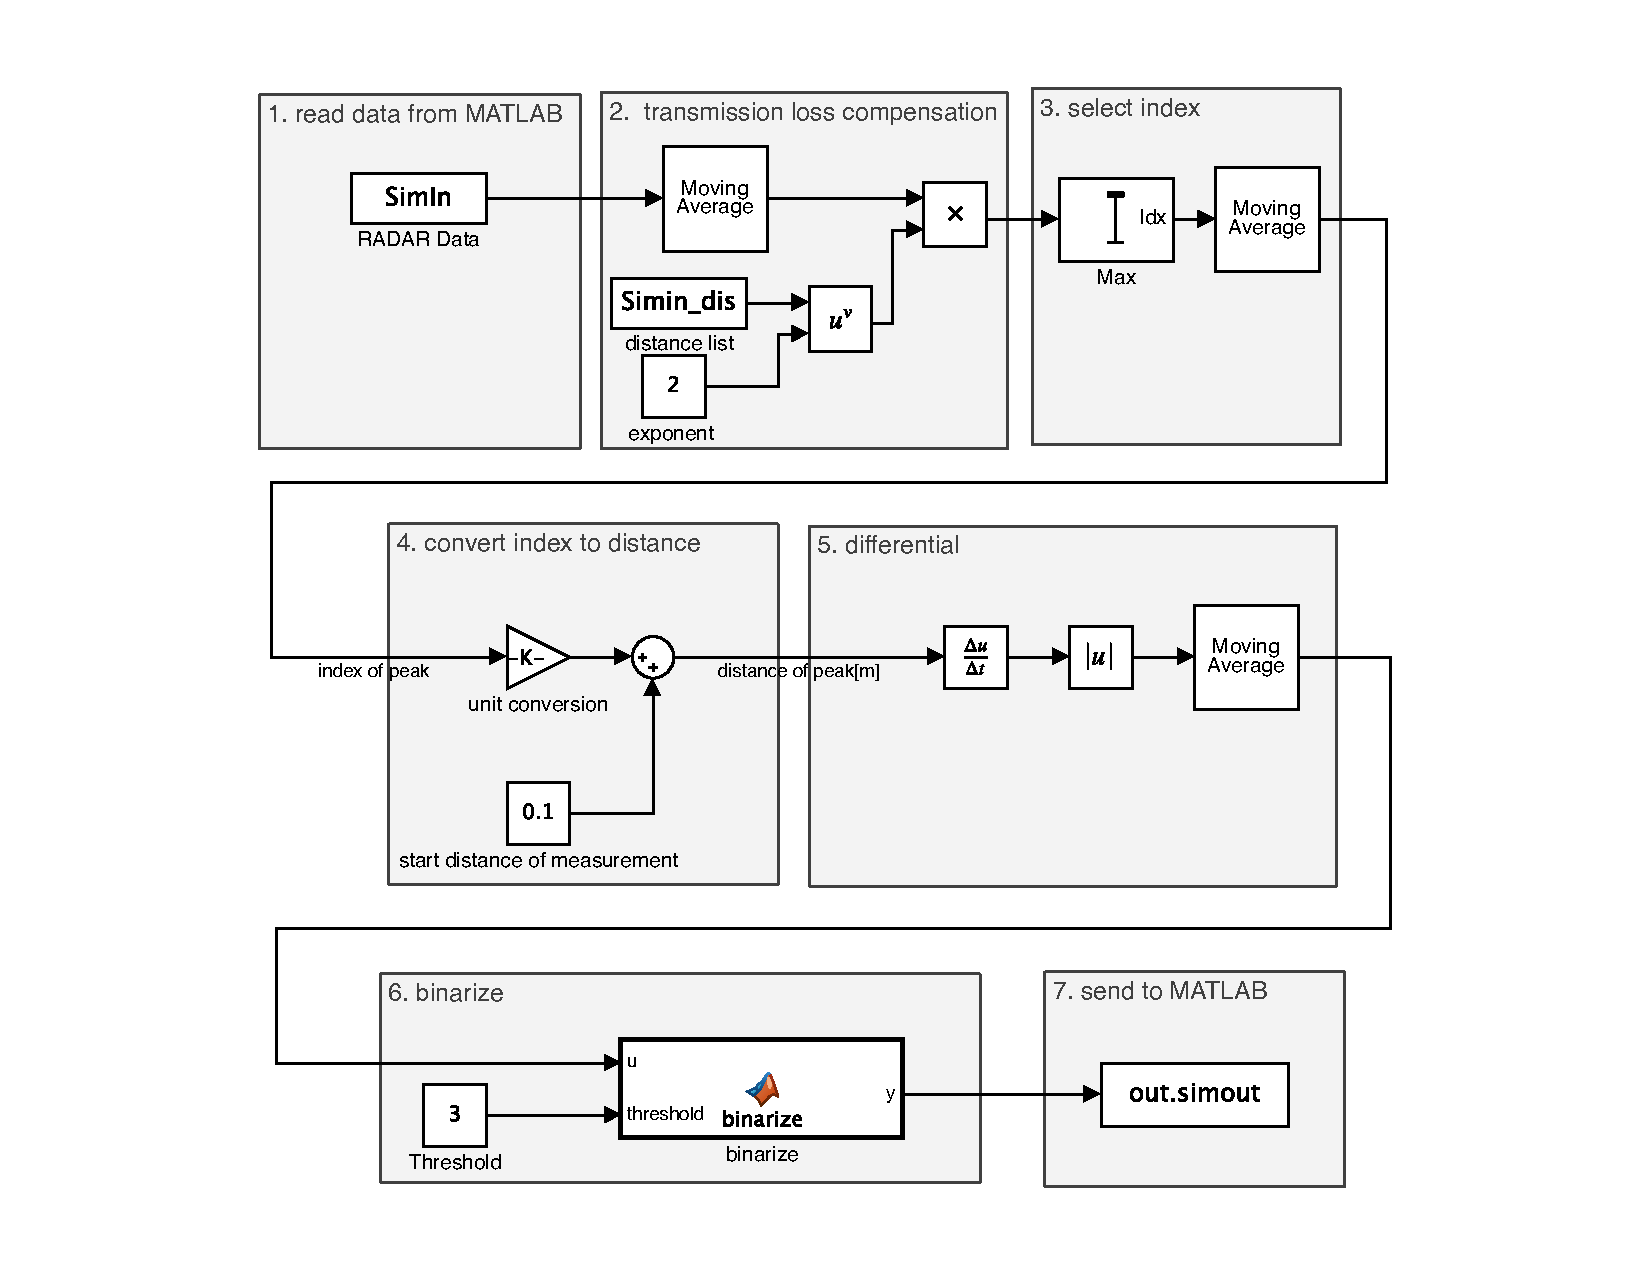
\includegraphics[width=8cm]{../thesis/fig/System_Block_BW.pdf}
  \caption{システムブロック図}
  \label{fig:system_block}
\end{figure}



\section{結言}
 

 ああああああああああああああああああああああああああああああああああああああああああああああああああああああああああああああああああああああああああああああああああああああああああああああああああああああああああああああああああああああああああああああああああああああああああああああああああああああああああああああああああああああああああああああああああああああああああああああああああああああああああああああああああああああああああああああああああああああああああああああああああああああああああああああああああああああああああああああああああああああああああああああああああああああああああああああああああああああああああああああああああああああああああああああああああああああああああああああああああああああああああああああああああああああああああああああああああああああああああああああああああああああああああああああああああああああああああああああああああああああああああああああああああああああああああああああああああああああああああああああああああああああああああああああああああああああああああああああああああああああああああああああああああああああああああああああああああああああああああああああああああああああああああああああああああああああああああああああああああああああああああああああああああああああああああああああああああああああああああああああああああああああああああああああああああああああああああああああああああああああああああああああああああ

\end{multicols}
\end{document}
